\documentclass[11pt,a4paper]{article}
\usepackage[T1]{fontenc}
\usepackage{lmodern}
\usepackage[a4paper,margin=2cm,headheight=14pt]{geometry}
\usepackage{amsmath,amssymb,bm}
\usepackage{booktabs,tabularx,array,multirow}
\usepackage{graphicx}
\usepackage{float}
\usepackage{xcolor}
\usepackage[most]{tcolorbox}
\usepackage{tikz}
\usetikzlibrary{arrows.meta,positioning,fit,calc}
\usepackage[round,authoryear]{natbib}
\setcitestyle{square}
\usepackage{multicol}
\usepackage{fancyhdr}
\usepackage{enumitem}
\usepackage[labelfont=bf,labelsep=period,font=small]{caption}
\usepackage[hidelinks]{hyperref}

\setlength{\parindent}{0pt}
\setlength{\parskip}{3pt}
\setlist{nosep,leftmargin=*}
\numberwithin{table}{section}
\numberwithin{figure}{section}
\numberwithin{equation}{section}
\captionsetup[table]{position=top,skip=3pt}
\captionsetup[figure]{skip=4pt}

\pagestyle{fancy}
\fancyhf{}
\renewcommand{\sectionmark}[1]{\markboth{\thesection\quad #1}{}}
\renewcommand{\subsectionmark}[1]{\markright{\thesubsection\quad #1}}
\fancyhead[L]{\small\leftmark}
\fancyhead[R]{\small\rightmark}
\fancyfoot[C]{\thepage}
\renewcommand{\headrulewidth}{0.4pt}
\fancypagestyle{plain}{\fancyhf{}\fancyfoot[C]{\thepage}\renewcommand{\headrulewidth}{0pt}}

\newcommand{\para}[1]{\textbf{#1}\ }
\newtcolorbox{defbox}[1]{colback=blue!3,colframe=black!30,boxrule=0.4pt,arc=2pt,
  title={\textbf{#1}},coltitle=black,colbacktitle=black!6,fonttitle=\small,left=4pt,right=4pt,top=3pt,bottom=3pt}

\begin{document}

\begin{titlepage}
\centering
\vspace*{2.5cm}
{\large M.TECH PROJECT REPORT\par}
\vspace{2cm}
{\LARGE\bfseries Can Self-Attention Models Capture\\[4pt] Context Effects?\par}
\vspace{0.5cm}
{\large Higher-order context effects, a comparison with DeepHalo,\\ and a first look inside the models\par}
\vspace{2.2cm}
{\large Ajaz Hussain\par}
DA25M006\par
\vspace{1cm}
M.Tech, Data Science and Artificial Intelligence\\
Indian Institute of Technology Madras\par
\vspace{0.8cm}
Guide: Prof.\ Suryanarayana Sankagiri\par
\vfill
November 2026\par
\end{titlepage}

\pagenumbering{roman}
\section*{Abstract}
\addcontentsline{toc}{section}{Abstract}
\thispagestyle{plain}
When we choose something, we hardly ever look at it alone. Whether we like a hotel, a phone or a cup of coffee depends a lot on what else is shown next to it. This is called a \emph{context effect}, and it breaks the IIA assumption on which the multinomial logit and most ranking models are built. In choice models, every option gets a score called its utility, which tells how attractive the option is: the higher its utility, the more likely it is to be chosen. Models like CDM and LCL can capture context, but only the first-order part of it, where each other item (or the average of the slate) pushes the utility of an item up or down. Neural networks can in principle learn effects of any order, but there is very little careful work on whether they actually learn them from choice data.

In this project, we have tried to check whether a self-attention model learns context effects of a known order, and whether it does this better than DeepHalo (Zhang et al., NeurIPS 2025), a recent neural choice model designed to control the order of interactions. Our self-attention model is a small Transformer encoder with no positional encoding: three layers, width 32, two heads and a 64-unit feed-forward block (about 26,000 parameters), with a linear head that gives each item a utility and a softmax over the slate. For DeepHalo we use the quadratic version described in its paper, with four residual layers, embedding width 16 and eight heads (about 11,700 parameters). Both models are tuned in the same way and tested on synthetic data in which we plant context effects of order one, two and three with the same strength. Since we know the true utilities, we also know the best possible loss (the oracle), and we compare every model with control models that cannot see the context at all.

Over 30 seeds, both models do equally well on first-order linear (LCL) context and recover about 97\% of it. On second- and third-order effects, self-attention gets a lower test loss than DeepHalo on every single seed. It captures 16.8\% to 32.3\% of the part of the effect that the mean and standard deviation of the slate cannot explain, against 5.7\% to 9.8\% for DeepHalo. Within attention, depth helps more than width, and the advantage remains when we change the kernel used to generate the data, although an earlier advantage on similarity effects did not. No model reaches the oracle, but a training-size sweep shows that this is mainly a data problem: with 1,000,000 slates, self-attention captures 38.2\% to 53.1\% of the hard part (DeepHalo 15.8\% to 21.8\%), while below about 100,000 slates neither model does better than the simple mean-and-sd summary. On real data, we find no usable context in London travel-mode choice (LPMC) and a small but reliable context gain in Expedia hotel bookings, most of which comes from comparing each hotel with the others in the same search. There, after tuning, self-attention and DeepHalo perform about the same, and the size sweep tells us that higher-order effects would not be visible at Expedia's data size anyway. Finally, a first look inside the models shows that on LCL data every model recovers the true $\boldsymbol\theta$ and $A$ almost exactly (correlation 0.999), with self-attention simply averaging the slate, while on higher-order data the attention heads focus on the items that are close in the features defining the effect, also when the kernel shortcut is removed. A direct IIA test ranks the models in the same order as our loss-based metric. A first test of depth against order shows that two layers of self-attention are enough for effects of order 2 to 5, while attention without its feed-forward network learns very little context.

\clearpage
\tableofcontents\thispagestyle{plain}
\clearpage
\pagenumbering{arabic}

\section{Introduction}

\subsection{Everyday examples of context effects}\label{sec:1.1}

Let us start with a simple situation. A caf\'e sells coffee in two sizes, small at Rs~100 and large at Rs~200, and most people pick the small one. Now the caf\'e adds a medium cup at Rs~190. Almost nobody buys the medium, but many people now shift to the large, because for just Rs~10 more than the medium they get much more coffee. The large cup has not changed at all. Only the cups around it have changed, and that was enough to change what people chose. This is what we call a \textbf{context effect}: how much we like an option depends on the other options shown along with it.

This idea is much older than choice modelling. In his well-known paper ``Features of Similarity'', Tversky (1977) argued that even our sense of \emph{similarity} depends on context. He described each object as a set of features, and wrote the similarity of $a$ to $b$ as a contrast between the features they share and the features that separate them:

\begin{equation}
s(a, b) = \theta\, f(A \cap B) - \alpha\, f(A \setminus B) - \beta\, f(B \setminus A)
\end{equation}

The important point is that the weights on the features are not fixed. According to his \emph{diagnosticity principle}, a feature becomes more important when it helps us divide the objects in front of us into groups. In one of his experiments, people were asked which country is most similar to Austria. When the options were Sweden, Poland and Hungary, 49\% chose Sweden. When Poland was replaced by Norway, only 14\% chose Sweden. Austria and Sweden were exactly the same in both cases; only the third country changed, and with it the way people grouped the countries in their mind.

Goldstone, Medin and Halberstadt (1997) showed that this happens even when people compare just two things: which features matter in the comparison changes with the other objects shown on the screen.

We should also be a little careful here. When Evers and Lakens (2014) repeated Tversky's study, they found only a small effect, and it disappeared once they ruled out a simpler explanation. So context effects are real, but they can be small, and something that looks like a context effect may have a different cause. This lesson matters for our project as well.

\subsection{Context effects in choice}\label{sec:1.2}

When people choose between options, three context effects have been reported again and again:

\begin{itemize}
\item \textbf{Attraction (decoy) effect} (Huber, Payne and Puto, 1982): adding an option that is clearly worse than one alternative, but not worse than the others, increases the share of the alternative it resembles. The coffee example above is of this kind.
\item \textbf{Compromise effect} (Simonson, 1989): an option lying between two extremes is chosen more often than when it is itself an extreme. For example, many of us pick the mid-range phone simply because it sits between a cheap one and a very expensive one.
\item \textbf{Similarity effect} (Tversky, 1972): a new option takes its share mostly from the options that are similar to it. In elections this is known as vote splitting.
\end{itemize}

All three break a rule called \textbf{independence of irrelevant alternatives (IIA)}, given by Luce (1959). It says that the ratio of the chances of choosing $i$ and $j$ should not depend on what else is offered:

\begin{equation}
\frac{P(i \mid S)}{P(j \mid S)} = \frac{P(i \mid S')}{P(j \mid S')} \quad \text{for every } S' \supseteq \{i, j\}
\end{equation}

The multinomial logit (MNL), which is the most widely used choice model, follows IIA by construction, and so does any ranking model that scores each item on its own. As Seshadri, Peysakhovich and Ugander (2019) point out, if we assume IIA when it does not actually hold, our predictions for new choice sets can go badly wrong.

Context effects can also act on features, and not only on particular products. Tomlinson and Benson (2021) give a nice example of a person choosing a restaurant. Among expensive restaurants, the person may care a lot about the wine list, while among fast-food places the same person may care more about how quickly the food comes. So the importance of a feature depends on the features of the whole choice set. They call this a \emph{feature context effect}.

\subsection{The order of a context effect}\label{sec:1.3}

A useful way to organise context effects is to break the utility of an item $j$ in a choice set $S$ into pieces, according to how many other items each piece depends on (Batsell and Polking, 1985; Seshadri et al., 2019; Zhang et al., 2025):

\begin{equation}
u_j(S) = v_j(\varnothing) + \sum_{k \in S \setminus j} v_j(\{k\}) + \sum_{\{k, l\} \subseteq S \setminus j} v_j(\{k, l\}) + \cdots + v_j(S \setminus j)
\end{equation}

Here $v_j(\varnothing)$ is the item's own value without any context. The first-order terms $v_j(\{k\})$ tell us how one other item $k$ changes the utility of $j$. The second-order terms $v_j(\{k,l\})$ tell us how a pair of items acts together, beyond what each does alone, and so on. The three effects above fit nicely into this picture (Zhang et al., 2025): the attraction effect is a positive first-order term, the similarity effect is a negative first-order term, and the compromise effect is a positive second-order term, because an option can be a ``compromise'' only with respect to \emph{two} extremes. MNL keeps only the zeroth-order term, while CDM and LCL add the first-order terms. Anything of order two or more needs a more flexible model. Once these utilities are known, the choice probability is again the softmax over the slate, $P(j\mid S)=\exp u_j(S)\big/\sum_{k\in S}\exp u_k(S)$ (Section 3.2). (A small note on naming: Seshadri et al. also count the target item itself, so they call the CDM a second-order model. In this report, the order always counts only the \emph{other} items, as in DeepHalo.)

\subsection{Can self-attention learn context effects?}\label{sec:1.4}

Transformers are now widely used to re-rank lists of items, because self-attention lets every item in a list look at every other item. So it is natural to expect that self-attention can model context effects of any order. But being able to represent something is not the same as actually learning it from data, and good accuracy alone does not prove that the model has learned context. The accuracy can come from the item's own features, or from things like the position of the item on the page. We saw this ourselves in our early experiments on Expedia hotel searches, where a model that used only position bias got an NDCG@10 of 0.3922, slightly better than the 0.3848 of the full attention model. Just like in the study of Evers and Lakens (2014), we have to separate a real effect from the things that can look like it.

So in this project we ask two questions:

\begin{enumerate}
\item \textbf{RQ1.} When a self-attention model is trained only on observed choices, which orders of context effect does it learn, and how much of each?
\item \textbf{RQ2.} Does it learn them better than DeepHalo, a model built specially to control the order of context effects?
\end{enumerate}

We answer both mainly on synthetic data, where we know the true utilities and therefore the best possible loss.

\subsection{The two models we compare}\label{sec:1.5}

Our \textbf{self-attention model} is a Transformer encoder that treats the choice set as a set, without any order. Each item's feature vector first goes through a linear layer and layer normalisation. Then come three encoder layers. Each layer has two-head self-attention followed by a small two-layer ReLU feed-forward network, and both parts have a residual connection followed by layer normalisation (the ``post-norm'' arrangement). The width is 32 and the feed-forward hidden size is 64. At the end, a linear head gives each item a utility, and a softmax over the slate gives the choice probabilities. We use no positional encoding, so shuffling the items does not change their scores. We also use a \emph{blindfolded twin} of this model, in which each item can attend only to itself. It cannot see the context at all, so it works as our context-free control. The full equations are given in Section 5.

\textbf{DeepHalo} (Zhang et al., 2025) builds the utility layer by layer, and each layer is designed to add one more order of interaction. Each item is first embedded by a shared three-layer network. In every layer, the model makes a summary of the slate by averaging a projection of all the items into $H$ ``interaction heads''. Then each item receives, for every head, a nonlinear function of its own original embedding multiplied by that head's summary. In the quadratic version, the item representations go through a quadratic activation before averaging, so the order that can be reached doubles with every layer. Our tuned DeepHalo has four layers, embedding width 16 and eight heads. The full equations are given in Section 6.
\begin{figure}[H]
\centering
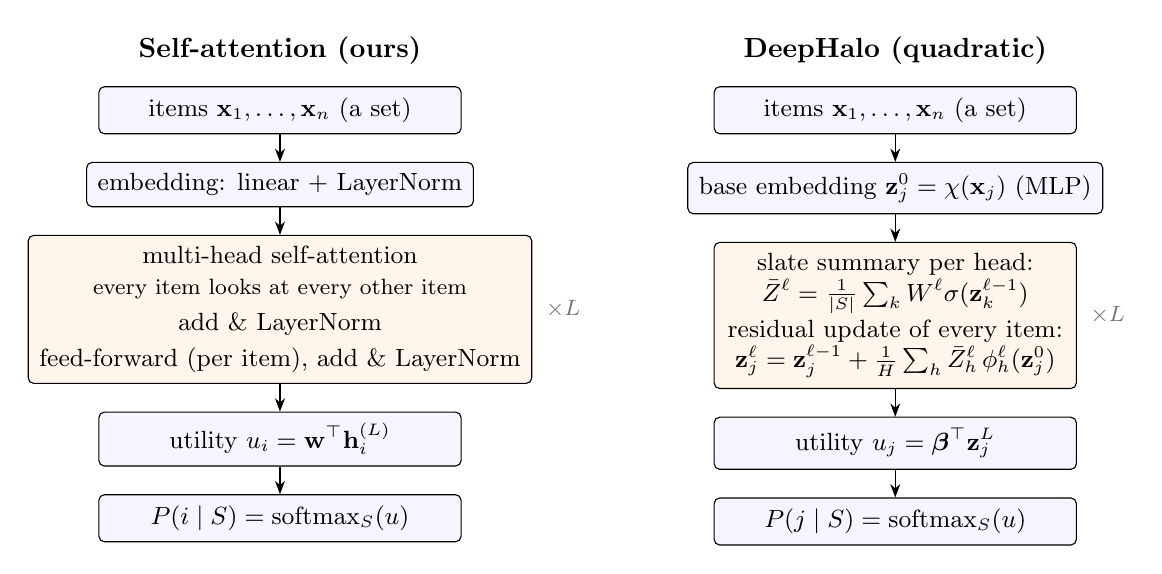
\begin{tikzpicture}[font=\small, box/.style={draw,rounded corners=2pt,fill=blue!4,align=center,minimum width=4.6cm,inner sep=4pt},
  lab/.style={font=\footnotesize\itshape,text=black!55}, >=Stealth]
% self-attention
\node[box] (sx) {items $\mathbf x_1,\dots,\mathbf x_n$ (a set)};
\node[box,below=0.35cm of sx] (se) {embedding: linear + LayerNorm};
\node[box,below=0.35cm of se,fill=orange!8] (sa) {multi-head self-attention\\ \footnotesize every item looks at every other item\\[2pt] add \& LayerNorm\\[2pt] feed-forward (per item), add \& LayerNorm};
\node[box,below=0.35cm of sa] (su) {utility $u_i=\mathbf w^{\top}\mathbf h^{(L)}_i$};
\node[box,below=0.35cm of su] (sp) {$P(i\mid S)=\mathrm{softmax}_S(u)$};
\draw[->] (sx)--(se); \draw[->] (se)--(sa); \draw[->] (sa)--(su); \draw[->] (su)--(sp);
\node[lab,right=0.05cm of sa] {$\times L$};
\node[above=0.15cm of sx,font=\bfseries] {Self-attention (ours)};
% deephalo
\node[box,right=3.2cm of sx] (dx) {items $\mathbf x_1,\dots,\mathbf x_n$ (a set)};
\node[box,below=0.35cm of dx] (de) {base embedding $\mathbf z^0_j=\chi(\mathbf x_j)$ (MLP)};
\node[box,below=0.35cm of de,fill=orange!8] (da) {slate summary per head:\\ $\bar Z^{\ell}=\frac1{|S|}\sum_k W^{\ell}\sigma(\mathbf z^{\ell-1}_k)$\\[2pt] residual update of every item:\\ $\mathbf z^{\ell}_j=\mathbf z^{\ell-1}_j+\frac1H\sum_h\bar Z^{\ell}_h\,\phi^{\ell}_h(\mathbf z^0_j)$};
\node[box,below=0.35cm of da] (du) {utility $u_j=\bm\beta^{\top}\mathbf z^L_j$};
\node[box,below=0.35cm of du] (dp) {$P(j\mid S)=\mathrm{softmax}_S(u)$};
\draw[->] (dx)--(de); \draw[->] (de)--(da); \draw[->] (da)--(du); \draw[->] (du)--(dp);
\node[lab,right=0.05cm of da] {$\times L$};
\node[above=0.15cm of dx,font=\bfseries] {DeepHalo (quadratic)};
\end{tikzpicture}
\caption{The two architectures compared in this report (full equations in Sections~5.1 and~6). In self-attention each item forms its own weights over the other items; in DeepHalo every item sees the same $H$ averaged numbers per layer and differs only in how its own base embedding responds to them.}\label{fig:arch}
\end{figure}

\subsection{Contributions and organisation}\label{sec:1.6}

The main contributions of this work are:

\begin{itemize}
\item We build a synthetic benchmark with context effects of order one, two and three, calibrated so that the part of each effect that simple slate statistics cannot explain has about the same size (about 0.03 nats).
\item We compare self-attention and DeepHalo carefully: both are tuned with the same budget, we use separate seeds for choosing models and for reporting results, and we add size-matched and context-blind control models.
\item We show that self-attention beats DeepHalo on second- and third-order effects on all 30 seeds, that within attention depth matters more than width, and that one advantage we saw earlier (on similarity effects) most likely came from the kernel used to generate the data.
\item We run a training-size sweep from 11,000 to 1,000,000 slates, which shows that the gap to the oracle is a data limit and that higher-order context cannot be learned below about 100,000 slates.
\item We apply the same models and controls to two real datasets, LPMC and Expedia, and find that the context we can detect there is shallow and mostly explained by simple slate statistics.
\end{itemize}

The rest of the report is organised as follows. Sections 2 to 4 build up the choice models, from Bradley--Terry to the first-order context models. Section 5 states our main question and describes the self-attention model. Section 6 describes DeepHalo, and Section 7 explains how we compare the two fairly. Section 8 gives our experiments and results, Section 9 discusses them, and Section 10 lists the future work.

\section{The simplest model: Bradley--Terry}

The Bradley--Terry (BT) model, proposed in 1952, is the simplest model for comparing two items. It gives each item $i$ a single number $u_i$, called its \textbf{utility} or score. A higher score means the item is liked more. When two items $i$ and $j$ are compared, the chance that $i$ wins is:

\begin{equation}
P(i \succ j) = \frac{e^{u_i}}{e^{u_i} + e^{u_j}} = \frac{1}{1 + e^{-(u_i - u_j)}}
\end{equation}

So only the \emph{difference} in scores matters. If both items have the same score, each wins half the time. If $i$ is better by a large margin, $i$ wins almost always.

\subsection{A small worked example}\label{sec:2.1}

Let us say tea has score $u_{\text{tea}}=1.0$ and coffee has score $u_{\text{coffee}}=0.0$. Then the chance of choosing tea over coffee is $1/(1+e^{-1})$, which is about 0.73. So in 100 such comparisons, we expect tea to win about 73 times. If we instead had $u_{\text{tea}}=2.0$, tea would win about 88 times out of 100.

This is exactly the same idea that is used in chess ratings (the Elo system) and, more recently, in ranking chatbot answers from human preferences. The scores are learned from data by maximum likelihood: we choose the scores that make the observed winners as likely as possible.

\subsection{Where Bradley--Terry falls short}\label{sec:2.2}

BT has two limitations for our problem:

\begin{itemize}
\item It handles only \textbf{pairs}. On a real website we choose one item out of many, not out of two.
\item Each item's score is \textbf{fixed}. Tea has the same score whether it is shown next to coffee, juice or a very bad tea. So BT cannot show any context effect at all.
\end{itemize}

The first limitation is removed by the multinomial logit model in the next section. The second one needs the context models of Sections 3 and 4.

\section{Multinomial logit and the universal logit}

\subsection{Multinomial logit (MNL)}\label{sec:3.1}

The multinomial logit (MNL) extends Bradley--Terry from two items to a whole slate $S$ of items. Each item still has a fixed score $u_i$, and the chance of choosing item $i$ from $S$ is a softmax over the slate:

\begin{equation}
P(i \mid S) = \frac{e^{u_i}}{\sum_{j \in S} e^{u_j}}
\end{equation}

When $S$ has only two items, this is exactly Bradley--Terry. In practice, the score is usually computed from the item's features. If item $i$ has a feature vector $\mathbf x_i$ (for example price, rating and distance for a hotel), we write $u_i=\boldsymbol\theta\cdot\mathbf x_i$, where $\boldsymbol\theta$ is a vector of learned weights.

Now let us see why MNL obeys IIA. Take any two items $i$ and $j$ in the slate. The ratio of their chances is:

\begin{equation}
\frac{P(i \mid S)}{P(j \mid S)} = \frac{e^{u_i}}{e^{u_j}} = e^{u_i - u_j}
\end{equation}

The denominator has cancelled out, so the ratio depends only on $i$ and $j$ and not on anything else in $S$. Adding or removing other items cannot change it. This is the IIA property, and it is why MNL cannot show the decoy, compromise or similarity effects from Section 1.

\subsection{The universal logit}\label{sec:3.2}

To allow context, we must let each item's score depend on the slate. We write $u_i(S)$ instead of $u_i$. The \textbf{universal logit} keeps the softmax form but allows any such slate-dependent score:

\begin{equation}
P(i \mid S) = \frac{e^{u_i(S)}}{\sum_{j \in S} e^{u_j(S)}}
\end{equation}

This is called ``universal'' because, for a fixed set of items, any choice behaviour at all can be written in this form. It is therefore too general to learn directly. The useful idea is to break $u_i(S)$ into pieces by \textbf{how many other items each piece depends on}.

\subsection{Orders of interaction}\label{sec:3.3}

We can expand the slate-dependent score as a sum of terms:

\begin{equation}
u_i(S) = \underbrace{u_i}_{\text{order 0}} + \underbrace{\sum_{j \in S \setminus i} u_{i \mid j}}_{\text{order 1}} + \underbrace{\sum_{\{j,k\} \subseteq S \setminus i} u_{i \mid jk}}_{\text{order 2}} + \underbrace{\sum_{\{j,k,l\} \subseteq S \setminus i} u_{i \mid jkl}}_{\text{order 3}} + \cdots
\end{equation}

In simple words:

\begin{itemize}
\item \textbf{Order 0} is the item's own value, with no context. Keeping only this term gives back MNL.
\item \textbf{Order 1} terms say how one other item $j$, on its own, pushes item $i$ up or down. For example, ``a cheap hotel nearby makes this hotel look expensive''.
\item \textbf{Order 2} terms say how a \emph{pair} of other items together affects $i$, beyond what each does alone. For example, item $i$ is helped only when it sits between two other items, which is the compromise effect.
\item \textbf{Order 3} terms involve a \emph{triple} of other items, and so on.
\end{itemize}

This view is very useful for our project. It turns the vague question ``does the model capture context?'' into a sharper one: \textbf{up to which order of interaction can the model capture context?} A model that only sees the average of the other items, for example, can represent order 1 well but will struggle with higher orders. We will design our synthetic datasets around exactly these orders in Section 8.

\section{First-order context models: CDM and LCL}

Both CDM and LCL keep only the order-0 and order-1 terms of the universal logit. They differ in how they describe the order-1 effect: CDM works with item identities, while LCL works with item features.

\subsection{Context-Dependent Model (CDM)}\label{sec:4.1}

The Context-Dependent Model of Seshadri, Peysakhovich and Ugander (ICML 2019) says that every other item $k$ in the slate gives a push $u_{ik}$ to item $i$. The pushes simply add up:

\begin{equation}
u_i(S) = \sum_{k \in S \setminus i} u_{ik}, \qquad u_{ik} = \mathbf{t}_i \cdot \mathbf{c}_k
\end{equation}

Here $\mathbf t_i$ is a ``target'' vector for item $i$ (how it is affected) and $\mathbf c_k$ is a ``context'' vector for item $k$ (how it affects others). Writing $u_{ik}$ as a dot product keeps the number of parameters small, since we do not need a separate number for every pair. The pushes need not be symmetric: a decoy can help the target a lot while the target does almost nothing to the decoy.

\subsection{Linear Context Logit (LCL)}\label{sec:4.2}

The Linear Context Logit of Tomlinson and Benson (KDD 2021) works with features, so it can handle new items that were never seen in training. Each item has a feature vector $\mathbf x_i$, and the slate is summarised by the \textbf{average feature vector} of its items, written $\bar{\mathbf x}_S$. The context then changes the weights $\boldsymbol\theta$ by a linear amount:

\begin{equation}
u_i(S) = \left(\boldsymbol{\theta} + A\, \bar{\mathbf{x}}_S\right) \cdot \mathbf{x}_i = \boldsymbol{\theta} \cdot \mathbf{x}_i + \mathbf{x}_i^\top A\, \bar{\mathbf{x}}_S
\end{equation}

The matrix $A$ is the heart of the model, and it is easy to interpret. The entry $A_{pq}$ says how the \emph{average} of feature $q$ in the slate changes how much people care about feature $p$. For example, if the hotels on the page are on average very expensive (feature $q$ = price), people may start caring more about the rating (feature $p$). If $A$ is all zeros, LCL becomes plain MNL.

Because $\bar{\mathbf x}_S$ is an average of the other items, each term in it depends on one other item at a time. So LCL is also a first-order model.

\subsection{What these models cannot do}\label{sec:4.3}

CDM and LCL are interpretable and work well on real data, but they assume that context acts through single items or through the average. They cannot express an effect that depends on two or three items \emph{together}, such as ``item $i$ gains only when it lies at the midpoint of two others''. This is exactly where more flexible neural models, like self-attention and DeepHalo, may help.

In our earlier work on this project, we trained self-attention on synthetic LCL data and checked whether it recovers the true $A$ and $\boldsymbol\theta$, not only the choices. That study found that training-set size matters much more for recovery than the rank or sparsity of $A$. This report builds on that work and moves to higher orders.


\subsection{Results of our earlier work on LCL data}\label{sec:4.4}

Since this report builds on our earlier study (the thesis in our GitHub repository, Section 5.3), we briefly summarise its main results here. That study looked only at first-order context. It asked whether a self-attention model trained on LCL data learns the true $A$ and $\boldsymbol\theta$, and not only good predictions. The data had $d=16$ features, $A$ of rank 5, five items per slate and 285,000 training sessions, and every comparison was repeated over 30 datasets. To read $A$ and $\boldsymbol\theta$ out of a trained model without looking at its weights, we used a \emph{behavioural probe}: it keeps two items fixed, refills the rest of the slate many times, and fits the LCL form of Section 4.2 to the change in their score gap. On the generator's own scores the probe is exact up to $10^{-15}$, and on a context-free model it returns zero.

\begin{table}[H]
\centering\small
\caption{Prediction and recovery on LCL data in our earlier study (30 datasets, mean; $\pm$ s.d.\ for the error). Excess NLL and KL are in units of $10^{-3}$. Error $=\lVert\hat A-A\rVert/\lVert A\rVert$; size $=\lVert\hat A\rVert/\lVert A\rVert$.}\label{tab:thesis}
\begin{tabular}{@{}lcccccc@{}}
\toprule
& \multicolumn{2}{c}{Prediction} & \multicolumn{3}{c}{Recovery of $A$} & $\boldsymbol\theta$\\
\cmidrule(lr){2-3}\cmidrule(lr){4-6}\cmidrule(l){7-7}
Model & Excess NLL & KL & Error & Cosine & Size & Rel.\ error\\
\midrule
Oracle LCL & 0.00 & 0.69 & 0.092 $\pm$ 0.010 & 0.996 & 1.01 & 0.020\\
Self-attention, 1 layer & 4.78 & 5.37 & 0.150 $\pm$ 0.040 & 0.990 & 0.93 & 0.042\\
Self-attention, 6 layers & 4.50 & 5.38 & 0.163 $\pm$ 0.062 & 0.987 & 0.93 & 0.046\\
Mean-pool, 2 layers & 4.14 & 4.72 & 0.142 $\pm$ 0.016 & 0.991 & 0.95 & 0.032\\
Flat MLP, 2 layers & 22.06 & 22.51 & 0.241 $\pm$ 0.035 & 0.979 & 0.85 & 0.026\\
\bottomrule
\end{tabular}
\end{table}

\begin{figure}[H]
\centering
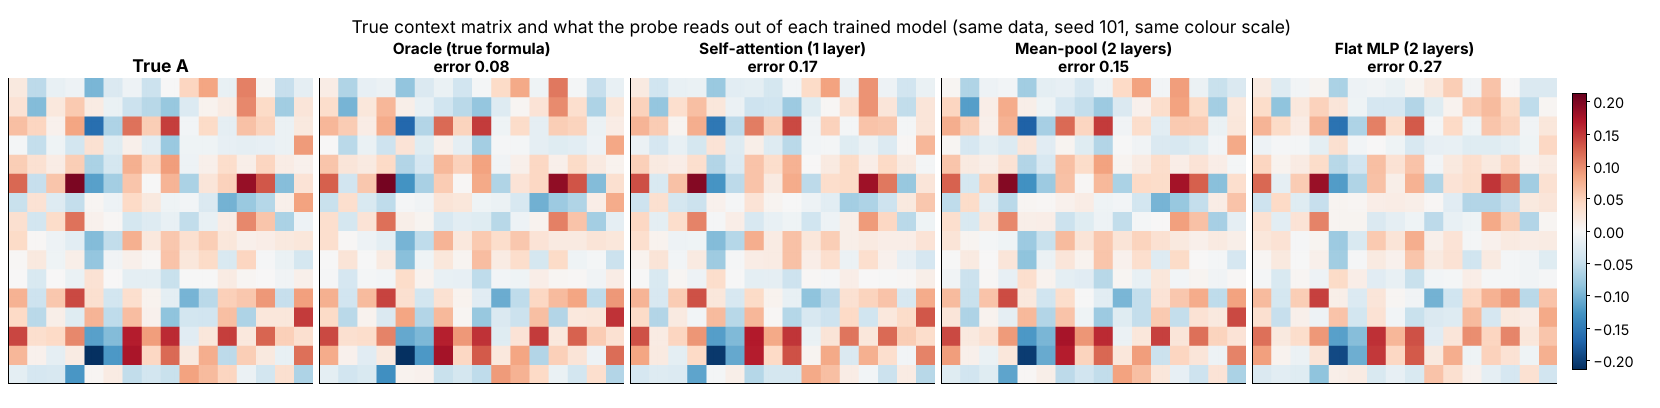
\includegraphics[width=0.85\textwidth]{figs/thesis_A_heatmaps.png}
\caption{The true $A$ of one LCL dataset and the $\hat A$ read from each trained model, on the same colour scale (from our earlier study).}\label{fig:heat}
\end{figure}

So a self-attention model that predicts well has also learned the context rule (Table~\ref{tab:thesis}, Figure~\ref{fig:heat}). Its $\hat A$ has the right pattern (cosine 0.990) and about 93\% of the true strength, and its error is about 1.6 times that of the oracle, which knows the true LCL form. It is within noise of the mean-pool network and clearly better than a flat MLP that reads the items one after the other. When it is trained on data with no context effect, it reports $\lVert\hat A\rVert=0.033$, against 0.93 when the effect is present, so it does not invent context.

Recovery depended mostly on the amount of training data (Figure~\ref{fig:thesis-size}): the error of self-attention fell from 0.79 at 18,000 sessions to 0.090 at 1.14 million. The rank of $A$ and the number of features mattered much less (for self-attention the error grew from 0.098 at rank 1 to about 0.17 at rank 16), and depth, sparsity, learning rate and weight decay did not matter. About 40\% of the remaining squared error of self-attention came from the random initialisation: averaging the matrices of 20 trained models brought its error from 0.144 to 0.110. Finally, among models that fit the usual data equally well, those that recovered $A$ better also predicted unusual slates better (partial correlation 0.73).

\begin{figure}[H]
\centering
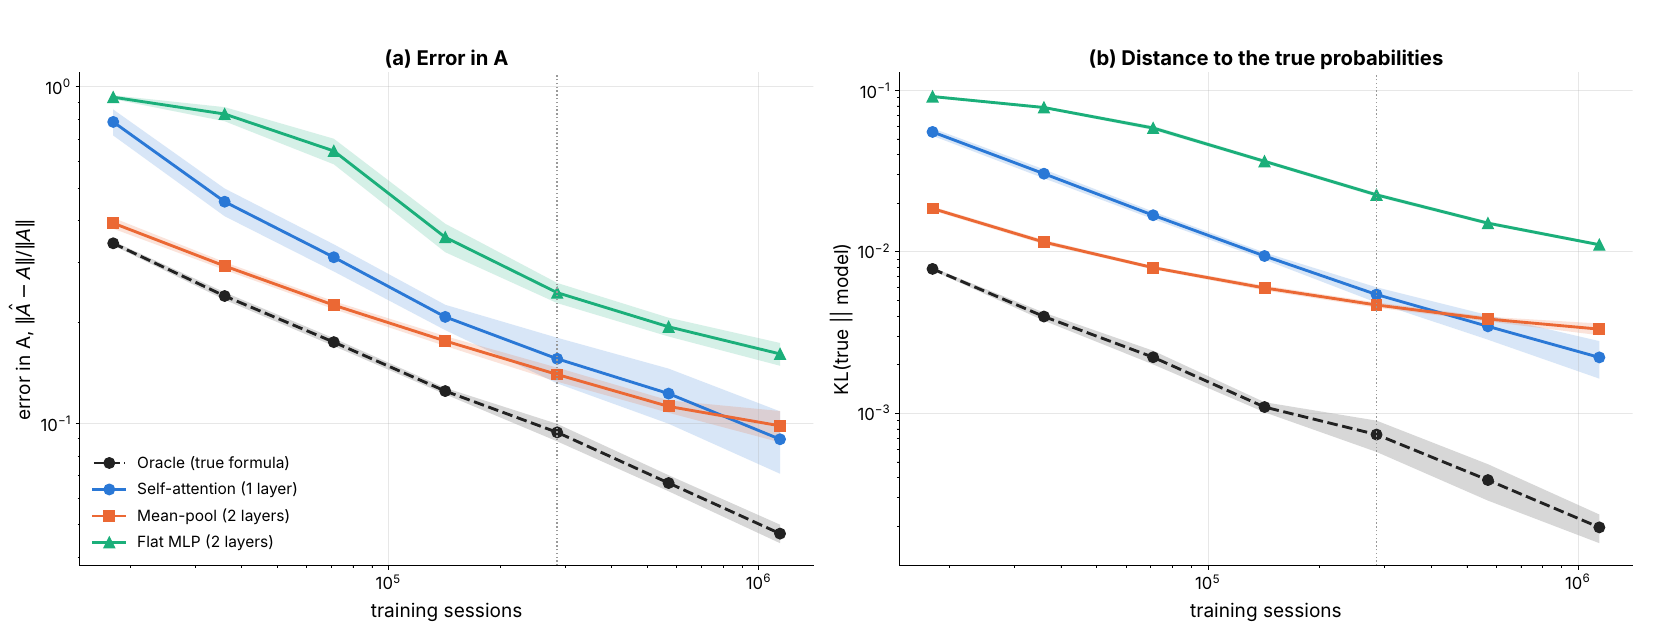
\includegraphics[width=0.8\textwidth]{figs/thesis_size.png}
\caption{LCL data, earlier study: error in $\hat A$ (a) and KL to the true probabilities (b) against the number of training sessions (log scales, 15 datasets per point; dotted line: reference size). Self-attention starts far behind but keeps improving and catches up with mean-pool at the largest sizes.}\label{fig:thesis-size}
\end{figure}


\section{The main question: can self-attention capture context effects?}

Our main question is: \textbf{when a self-attention model is trained only on observed choices, does it learn the context effects in the data, and up to which order?} Before answering this, let us see how self-attention is used for choice.

\subsection{Architecture of the self-attention model}\label{sec:5.1}

The model is a Transformer encoder (Vaswani et al., 2017) applied to the choice set $S=\{1,\dots,n\}$, where alternative $i$ has feature vector $\mathbf x_i\in\mathbb R^p$ ($p=6$ in all experiments). It has four parts.

\textbf{Embedding.} Each alternative is mapped linearly to width $d$ and layer-normalised:

\begin{equation}
\mathbf{h}_i^{(0)} = \mathrm{LN}\!\left(W_e \mathbf{x}_i + \mathbf{b}_e\right), \qquad W_e \in \mathbb{R}^{d \times p}
\end{equation}

No positional encoding is added, because a choice set has no natural order.

\textbf{Multi-head self-attention.} In layer $\ell$, each of $R$ heads forms queries, keys and values from the current representations, with head dimension $d_r=d/R$:

\begin{equation}
\mathbf{q}_i^{r} = W_Q^{r}\mathbf{h}_i^{(\ell-1)}, \quad \mathbf{k}_j^{r} = W_K^{r}\mathbf{h}_j^{(\ell-1)}, \quad \mathbf{v}_j^{r} = W_V^{r}\mathbf{h}_j^{(\ell-1)}, \qquad a_{ij}^{r} = \frac{\exp\!\big(\mathbf{q}_i^{r} \cdot \mathbf{k}_j^{r} / \sqrt{d_r}\big)}{\sum_{m \in S} \exp\!\big(\mathbf{q}_i^{r} \cdot \mathbf{k}_m^{r} / \sqrt{d_r}\big)}
\end{equation}

\begin{equation}
\mathrm{MHA}(\mathbf{h}^{(\ell-1)})_i = W_O \left[\, \textstyle\sum_{j \in S} a_{ij}^{1} \mathbf{v}_j^{1} \;;\; \cdots \;;\; \sum_{j \in S} a_{ij}^{R} \mathbf{v}_j^{R} \right]
\end{equation}

The weight $a^r_{ij}$ measures how much alternative $i$ draws on alternative $j$ in head $r$. This is the only operation in the network that mixes information across alternatives.

\textbf{Encoder layer (post-norm).} Attention and a position-wise feed-forward network are each wrapped in a residual connection followed by layer normalisation:

\begin{equation}
\tilde{\mathbf{h}}_i^{(\ell)} = \mathrm{LN}\!\left(\mathbf{h}_i^{(\ell-1)} + \mathrm{MHA}(\mathbf{h}^{(\ell-1)})_i\right), \qquad \mathbf{h}_i^{(\ell)} = \mathrm{LN}\!\left(\tilde{\mathbf{h}}_i^{(\ell)} + W_2\, \mathrm{ReLU}\!\big(W_1 \tilde{\mathbf{h}}_i^{(\ell)} + \mathbf{b}_1\big) + \mathbf{b}_2\right)
\end{equation}

The feed-forward network has hidden size $2d$ and acts on each alternative separately.

\textbf{Utility and choice.} After $L$ layers, a linear head gives each alternative a context-dependent utility, and a softmax over the choice set gives the choice probabilities, exactly in the form of the universal logit:

\begin{equation}
u_i(S) = \mathbf{w}^{\top} \mathbf{h}_i^{(L)} + b, \qquad P(i \mid S) = \frac{\exp u_i(S)}{\sum_{j \in S} \exp u_j(S)}
\end{equation}

The model is trained by minimising the negative log-likelihood of the observed choices. No dropout is used.

\begin{table}[H]
\centering\small
\caption{Settings of the tuned self-attention model.}\label{tab:0}
\begin{tabular}{@{}ll@{}}
\toprule
\textbf{Setting} & \textbf{Value used} \\
\midrule
Layers $L$ & 3 \\
Width $d$ & 32 \\
Heads $R$ & 2 (head dimension 16) \\
Feed-forward hidden size & 64 \\
Positional encoding & none \\
Normalisation & post-norm LayerNorm \\
Parameters & 25,953 \\
\bottomrule
\end{tabular}
\end{table}

These settings were not our first choice. Our first models had one or two layers; the values above were chosen later by tuning over 22 configurations of both models, using separate random seeds for choosing and for reporting (Section 7.2).

\textbf{Blindfolded twin.} The context-free control uses the same building blocks (one encoder layer, width 32, two heads), but the attention is masked so that $a^r_{ij}=0$ whenever $j\neq i$. Each alternative then attends only to itself, and its utility depends only on its own features. Any loss reduction of the full model over the twin must therefore come from context.

\subsection{Why it looks like a natural fit}\label{sec:5.2}

Self-attention has three properties that match choice problems well:

\begin{itemize}
\item \textbf{The order of items does not matter.} If we shuffle the slate, each item gets the same score. This is correct for choice, since a set of items has no natural order (we deliberately use no position encoding).
\item \textbf{Slates of any size can be used.} The same weights work for 5 items or 50 items.
\item \textbf{Every item can see every other item.} So, in principle, the score of item $i$ can depend on the whole slate, which is what the universal logit needs.
\end{itemize}

In fact, it is known that even one softmax attention layer with a feed-forward network can approximate any permutation-equivariant function, given enough width (Kajitsuka and Sato, 2024). So the question is not really whether attention \emph{can} represent context effects. The real questions are whether it \emph{learns} them from a finite amount of choice data, and how its depth relates to the order of effects it can learn.

\subsection{Accuracy is not the same as recovery}\label{sec:5.3}

A very important point in this project is that \textbf{good prediction does not prove that context was learned}. On real data, a model can get high accuracy for other reasons: the item's own features may explain most of the choices, or the model may use the item's position on the page. We saw this ourselves in early experiments on Expedia hotel data, where a model that used only position bias did slightly better (NDCG@10 of 0.3922) than full attention (0.3848). The code and notebooks of these earlier experiments, including our earlier LCL and CDM studies, are available in our GitHub repository: \href{https://github.com/ajazhsn/Ajaz_Hussain_MTP-}{\texttt{github.com/ajazhsn/Ajaz\_Hussain\_MTP-}}.

So in this project we mostly use \textbf{synthetic data}, where we plant a known context effect and know the true utilities. This lets us measure exactly how much of the planted effect each model recovers, and compare it with control models that are not allowed to see context at all.

\section{DeepHalo}

DeepHalo (Zhang, Wang, Gao and Li, NeurIPS 2025) is a neural choice model that uses item features while keeping explicit control over the order of the context effects it can represent. In cognitive science the influence of the choice set on preferences is also called the \emph{Halo effect}, which gives the model its name.

\subsection{Starting point: an order-wise decomposition}\label{sec:6.1}

DeepHalo extends the decomposition of Section 1.3 to feature-based utilities. Its Proposition 1 states that every permutation-equivariant utility function can be written as a sum over subsets of the other alternatives:

\begin{equation}
u_j(X_S) = \sum_{T \subseteq S \setminus \{j\}} v_j\!\left(X_{T \cup \{j\}}\right) = \sum_{p=0}^{|S|-1} \; \sum_{T \subseteq S \setminus \{j\},\, |T| = p} v_j\!\left(X_{T \cup \{j\}}\right)
\end{equation}

Here $X_{T\cup\{j\}}$ keeps the feature vectors of $j$ and of the subset $T$ and sets the others to zero, and the inner sum collects the p-th order interactions. The architecture is built so that successive layers add successively higher orders.

\subsection{The linear (recursive) form}\label{sec:6.2}

\textbf{Base embedding.} Every alternative is passed through a shared nonlinear embedding $\chi$, giving $\mathbf z_j^0=\chi(\mathbf x_j)\in\mathbb R^d$. In the released code, $\chi$ is a three-layer ReLU network followed by layer normalisation.

\textbf{Context summary.} At layer $\ell$, the current representations of all alternatives are projected into $H$ \emph{interaction heads} and averaged over the choice set:

\begin{equation}
\bar{Z}^{\ell} = \frac{1}{|S|} \sum_{k \in S} W^{\ell} \mathbf{z}_k^{\ell-1} \in \mathbb{R}^{H}, \qquad W^{\ell} \in \mathbb{R}^{H \times d} \qquad \text{(Eq. 4 of the paper)}
\end{equation}

The authors interpret the $H$ heads as $H$ consumer types with different tastes.

\textbf{Residual update.} Each alternative is updated by adding, for every head h, a nonlinear transformation of its own \emph{base} embedding scaled by that head's summary:

\begin{equation}
\mathbf{z}_j^{\ell} = \mathbf{z}_j^{\ell-1} + \frac{1}{H} \sum_{h=1}^{H} \bar{Z}_h^{\ell}\, \phi_h^{\ell}\!\left(\mathbf{z}_j^{0}\right) \qquad \text{(Eq. 5 of the paper)}
\end{equation}

In the released code, $\phi_h^{\ell}(\mathbf z)=\mathrm{LN}\big(W_2^{\ell}\,\mathrm{ReLU}(W_{1,h}^{\ell}\mathbf z+\mathbf b_{1,h}^{\ell})+\mathbf b_2^{\ell}\big)$, with a separate first layer for each head and a shared second layer.

\textbf{Utility and choice.} After $L$ layers, $u_j(X_S)=\boldsymbol\beta^{\top}\mathbf z_j^L$, and the choice probabilities are the softmax of these utilities over the choice set, as in the universal logit.

Because each layer multiplies a summary of the previous layer by a function of the base embedding, each layer raises the attainable order by one: the $\ell$-th layer captures interactions up to order $\ell$, and $L$ layers reach order $L$. The residual connection keeps the lower-order effects built by earlier layers.

\subsection{The quadratic form}\label{sec:6.3}

Reaching high orders with Eq. 4 requires one layer per order. To grow the order faster, the paper replaces the linear aggregation with a \emph{polynomial} one, passing each representation through an element-wise polynomial activation $\sigma$ before averaging:

\begin{equation}
\bar{Z}^{\ell} = \frac{1}{|S|} \sum_{k \in S} W^{\ell}\, \sigma\!\left(\mathbf{z}_k^{\ell-1}\right)
\end{equation}

With a quadratic $\sigma$, the order of the representation doubles at every layer. In the featureless setting the paper shows that an L-layer network with $\sigma(\cdot)=(\cdot)^2$ represents interactions up to order $2^{L-1}$, so that about $\log_2 J$ layers suffice for all orders among $J$ alternatives. Its synthetic experiment supports this: at a fixed parameter count, error falls sharply as depth grows until $2^{L-1}$ exceeds the choice-set size, and extra width does not make up for insufficient depth.

\begin{table}[H]
\centering\small
\caption{Highest order of interaction that $L$ layers of DeepHalo can reach.}\label{tab:1}
\begin{tabular}{@{}lll@{}}
\toprule
\textbf{Layers $L$} & \textbf{Highest order, linear form (Eq. 4)} & \textbf{Highest order, quadratic form (Eq. 6)} \\
\midrule
1 & 1 & 1 \\
2 & 2 & 2 \\
3 & 3 & 4 \\
4 & 4 & 8 \\
\bottomrule
\end{tabular}
\end{table}

\subsection{Implementation used in this work}\label{sec:6.4}

The authors' released code implements the linear form (Eqs. 4 and 5). It also defines two linear maps intended for the quadratic activation, but never applies them. Our first round of experiments used the released code unchanged, and therefore the linear form. Since the quadratic form is the one the paper proposes for higher-order effects, we then wired those two maps into the aggregation and refer to the result as \textbf{DHQ}:

\begin{equation}
\sigma(\mathbf{z}) = \left(A\mathbf{z} + \mathbf{a}\right) \odot \left(B\mathbf{z} + \mathbf{b}\right), \qquad \bar{Z}^{\ell} = \frac{1}{|S|} \sum_{k \in S} W^{\ell}\, \sigma\!\left(\mathbf{z}_k^{\ell-1}\right)
\end{equation}

Here $\odot$ is the element-wise (Hadamard) product, and $A$, $B$ are shared across layers, as in the released code. This is a learnable quadratic activation that contains the square $(\cdot)^2$ used in the paper as a special case. The embedding, the modulators $\phi$, the residual update (Eq. 5) and the output layer are the authors' code without change. Unless stated otherwise, all DeepHalo results in Section 8 use DHQ.

\begin{table}[H]
\centering\small
\caption{Settings of the tuned DeepHalo model (DHQ).}\label{tab:2}
\begin{tabular}{@{}ll@{}}
\toprule
\textbf{Setting} & \textbf{Value used} \\
\midrule
Layers $L$ & 4 \\
Embedding width $d$ & 16 \\
Interaction heads $H$ & 8 \\
Aggregation & quadratic (DHQ, Eq. 6) \\
Parameters & 11,713 \\
\bottomrule
\end{tabular}
\end{table}

Like the self-attention settings, this configuration was not fixed in advance. We first ran the paper's own configuration ($L=4$, $d=32$, $H=8$) and smaller variants, and the values above were then chosen by the same tuning procedure as for self-attention (Section 7.2).

\subsection{How DeepHalo differs from self-attention}\label{sec:6.5}

The two architectures mix information across alternatives in different ways. In DeepHalo, context enters through the averages $\bar Z_h^{\ell}$: every alternative sees the same $H$ numbers per layer, and differs only in how its own base embedding responds to them. In self-attention, each alternative $i$ forms its own weights $a_{ij}$ over the others, so the information it receives depends on how it relates to each other alternative individually. Whether this difference explains the results of Section 8 is still an open question.

\section{Comparing self-attention with DeepHalo fairly}

The second question of this report is whether self-attention captures context effects \textbf{better than DeepHalo}. Comparing two neural networks sounds easy, but it is very easy to get a misleading answer. One model may simply have more parameters, may have been tuned more carefully, or may be lucky on one random seed. We took the following steps to avoid these problems.

\subsection{Same data, same training}\label{sec:7.1}

Both models see exactly the same training, validation and test slates. Both are trained with the same recipe: the Adam optimiser with learning rate $10^{-3}$, then $10^{-4}$ for fine-tuning, batch size 512, and early stopping on the validation loss. The final numbers are always reported on a separate test set that was never used for any decision.

\subsection{Tuning both models equally}\label{sec:7.2}

We tuned both architectures over a grid of depths and widths: 22 configurations in total across the two families, on 7 datasets. To avoid the ``winner's curse'' (picking a configuration that only looked good by chance), we chose the best configuration using one set of random seeds (100 to 104) and then reported results on a completely different set of 30 seeds (0 to 29). The chosen configurations were:

\begin{table}[H]
\centering\small
\caption{Configurations chosen by tuning.}\label{tab:3}
\begin{tabular}{@{}lllll@{}}
\toprule
\textbf{Model} & \textbf{Layers} & \textbf{Width} & \textbf{Heads} & \textbf{Parameters} \\
\midrule
Self-attention (tuned) & 3 & 32 & 2 & about 26,000 \\
DeepHalo, quadratic (tuned) & 4 & 16 & 8 & about 11,700 \\
\bottomrule
\end{tabular}
\end{table}

The tuned DeepHalo has fewer parameters. So, separately, we also ran \textbf{size controls}, where the two families are matched more closely in parameter count, to make sure that any gap is not just because of size.

\subsection{Control models}\label{sec:7.3}

To know whether a model has really learned \emph{context}, we compare it with control models that are deliberately limited:

\begin{itemize}
\item \textbf{Oracle.} It uses the true utilities that generated the data. Since choices are random, even the oracle has some loss; this loss is the floor that no model can beat.
\item \textbf{Blindfolded twin.} This is the same attention model, but each item is only allowed to attend to itself. It can learn everything about an item's own features but nothing about the other items. Any improvement over the twin must come from context.
\item \textbf{Mean+sd pool.} Each item sees its own features plus only the \textbf{mean and standard deviation} of the other items in the slate. This is a cheap summary of the context. If a model beats this pool, it has learned something about context that a simple summary cannot give.
\end{itemize}

\subsection{Paired comparison over seeds}\label{sec:7.4}

For every seed, both models are trained on the same data, so we can compare them seed by seed. We report how many of the 30 seeds each model wins, along with the average difference and its standard error. A result like ``30 out of 30'' means one model was better on every single seed, which is very strong evidence.

\section{Experiments and results}

The headline result is that self-attention and DeepHalo tie on first-order linear context, while on second- and third-order context the tuned self-attention model beats the tuned DeepHalo model on all 30 seeds. Below we first describe the data and the metrics, and then go through the results one by one.

\subsection{Synthetic datasets}\label{sec:8.1}

Every slate has 10 items, and every item has 6 features drawn at random. The true utility of each item is its own part, $\boldsymbol\theta\cdot\mathbf x_i$, plus a context part of a chosen order. The context part uses only the first two features, so that we can picture the items as points on a 2-D plane. Each dataset has 285,000 training slates, 15,000 validation slates and 50,000 test slates, and the chosen item is sampled from the true choice probabilities.

\begin{table}[H]
\centering\small
\caption{The synthetic datasets.}\label{tab:4}
\begin{tabularx}{\textwidth}{@{}ll>{\raggedright\arraybackslash}X>{\raggedright\arraybackslash}X@{}}
\toprule
\textbf{Dataset} & \textbf{Order} & \textbf{What the context part rewards (or punishes)} & \textbf{Real-life analogue} \\
\midrule
D0 (LCL) & 1, linear & $\mathbf x_i^{\top}A\,\bar{\mathbf x}_S$, exactly the LCL model & Average price on the page changes how much people care about rating \\
D1 (similarity) & 1, nonlinear & Item $i$ loses utility for every other item close to it & Similarity effect: look-alikes steal from each other \\
D2 (compromise) & 2 & Item $i$ gains when it is close to the midpoint of a pair of other items & Compromise effect: the middle option wins \\
D3 (centre) & 3 & Item $i$ gains when it is close to the centre of a triple of other items & A higher-order version of the compromise effect \\
\bottomrule
\end{tabularx}
\end{table}

For D1 to D3, ``close'' is measured with a Gaussian kernel, $\exp(-d^2/\sigma^2)$ with $\sigma=0.2$, where $d$ is the distance on the 2-D plane. To check that our conclusions do not depend on this choice, we also built \textbf{box-kernel} versions D1b, D2b and D3b, where ``close'' simply means within a distance of 0.25 (Section 8.6).

\textbf{How the data is generated.} In every dataset, each slate $S$ has $n=10$ items, and the feature vector $\mathbf x_i$ of each item has 6 entries drawn independently from a standard normal distribution. For each random seed, a weight vector $\boldsymbol\theta$ is drawn at random and scaled to length 1. The true utility of item $i$ is its own part plus a planted context part, and the chosen item is drawn from the softmax of these utilities:

\begin{equation}
u_i(S) = \boldsymbol{\theta} \cdot \mathbf{x}_i + s\, \lambda\, c_i(S), \qquad P(i \mid S) = \frac{\exp u_i(S)}{\sum_{j \in S} \exp u_j(S)}
\end{equation}

Here $c_i(S)$ is the context term, which is different for each dataset, $\lambda$ sets its strength (Section 8.2) and $s=+1$ or $-1$ sets its sign.

\emph{LCL (D0).} The context term is exactly the LCL model of Section 4.2:

\begin{equation}
c_i(S) = \mathbf{x}_i^{\top} A\, \bar{\mathbf{x}}_S, \qquad \bar{\mathbf{x}}_S = \frac{1}{n} \sum_{j \in S} \mathbf{x}_j
\end{equation}

where $\bar{\mathbf x}_S$ is the mean of all items in the slate. For each seed, $A=UV^{\top}$ with $U$ and $V$ random $6\times2$ matrices, so $A$ has rank 2, and $A$ is scaled so that its Frobenius norm is 1.

\emph{Higher-order datasets (D1 to D5 and the box versions).} Only the first two features are used for context; we call them the item's position $\mathbf p_i=(x_{i1},x_{i2})$ on a 2-D plane. For an effect of order $k$, the context term adds up, over every group $T$ of $k$ other items, how close item $i$ is to the centre of that group:

\begin{equation}
c_i(S) = \sum_{T \subseteq S \setminus \{i\},\ |T| = k} K\!\left( \big\lVert \mathbf{p}_i - \bar{\mathbf{p}}_T \big\rVert^2 \right), \qquad \bar{\mathbf{p}}_T = \frac{1}{k} \sum_{j \in T} \mathbf{p}_j
\end{equation}

Each term depends jointly on item $i$ and the $k$ items in $T$, so the effect is of order $k$. The closeness $K$ is either the Gaussian kernel $K(d^2)=\exp(-d^2/\sigma^2)$ with $\sigma=0.2$, or, in the box versions, $K(d^2)=1$ if $d<0.25$ and 0 otherwise. For $k=1$ the centre of a group is just the other item itself, so the term measures how close item $i$ is to each other item.

\begin{table}[H]
\centering\small
\caption{Order, sign and strength $\lambda$ of the planted context term.}\label{tab:5}
\begin{tabularx}{\textwidth}{@{}llll>{\raggedright\arraybackslash}X@{}}
\toprule
\textbf{Dataset} & \textbf{Order $k$} & \textbf{Sign $s$} & \textbf{$\lambda$} & \textbf{What it means} \\
\midrule
D0 (LCL) & 1, linear & +1 & 1.3120 & The slate mean changes how much each feature is valued \\
D1 (similarity) & 1 & $-$1 & 1.8310 & An item loses utility for every look-alike in the slate \\
D2 (compromise) & 2 & +1 & 0.5087 & An item gains when it lies between two other items \\
D3 (centre) & 3 & +1 & 0.2507 & An item gains when it lies at the centre of three other items \\
D4 & 4 & +1 & 0.1440 & Same, for groups of four (Section 8.14) \\
D5 & 5 & +1 & 0.1098 & Same, for groups of five (Section 8.14) \\
\bottomrule
\end{tabularx}
\end{table}

The box versions D1b, D2b and D3b use the same order and sign as D1, D2 and D3, with their own $\lambda$ chosen by the same rule. The values of $\lambda$ are fixed in the code, so every run uses exactly the same data for a given seed.

\subsection{Setting the strength of the effect}\label{sec:8.2}

If a planted effect is too strong, every model learns it; if it is too weak, no model can find it in the noise. So we scaled each dataset's context part with a factor $\lambda$. The key quantity is what we call the \textbf{hard part}: the amount of the context effect that cannot be explained by an item's own features plus the mean and standard deviation of the other items. We set $\lambda$ so that the hard part is about the same for all higher-order datasets, about 0.03 nats of loss (in the final runs, the mean+sd pool ends between 0.023 and 0.032 nats above the oracle). For D0, the total context effect (the gap between the twin and the oracle) is 0.05 nats. This makes the datasets comparable: a model's score on D2 and on D3 can be read on the same scale.

\subsection{Metrics}\label{sec:8.3}

Our basic measure is the \textbf{test cross-entropy}, the average of $-\log P(\text{chosen item}\mid\text{slate})$ on the test set; lower is better. Every model is compared with the oracle, the blindfolded twin and the mean+sd pool from Section 7.3. We use two percentages:

\begin{equation}
\text{Gap to twin closed} = \frac{\mathrm{CE}_{\text{twin}} - \mathrm{CE}_{\text{model}}}{\mathrm{CE}_{\text{twin}} - \mathrm{CE}_{\text{oracle}}} \times 100\%
\end{equation}

\begin{equation}
\text{Hard part captured} = \frac{\mathrm{CE}_{\text{pool}} - \mathrm{CE}_{\text{model}}}{\mathrm{CE}_{\text{pool}} - \mathrm{CE}_{\text{oracle}}} \times 100\%
\end{equation}

The first one tells us what fraction of the \emph{whole} context effect a model has recovered. The second one tells us what fraction of the \emph{hard part} it has recovered, that is, how much it learned beyond a simple mean+sd summary. A value of 100\% means the model is as good as the oracle, 0\% means it is no better than the control, and a negative value means it is worse.

Why does lower loss mean that context has been learned? For any two items $i$ and $j$, $\log P(i\mid S)-\log P(j\mid S)=u_i(S)-u_j(S)$. So a model can beat the twin only by getting the context-dependent part of these differences more right, averaged over all pairs and slates. The IIA test from Section 1 looks at the same quantity for one pair at a time.

\subsection{First-order linear context (D0, LCL)}\label{sec:8.4}

On D0, all the models tie. Self-attention, DeepHalo and even the simple mean+sd pool each close about \textbf{97\% of the gap to the twin}. This is expected: an LCL effect depends only on the average of the slate, which every one of these models can compute easily. So, on first-order linear context, there is \textbf{no advantage} for either architecture. This also tells us that the training pipeline works: when the effect is simple, all models find almost all of it.

\subsection{Higher-order context (D1, D2, D3 and their box versions)}\label{sec:8.5}

The picture changes completely once the effect is of higher order. On D2, D3, D2b and D3b, the tuned self-attention model has lower test loss than the tuned DeepHalo model \textbf{on all 30 seeds}. The share of the hard part each model captures is shown below.

\begin{figure}[H]
\centering
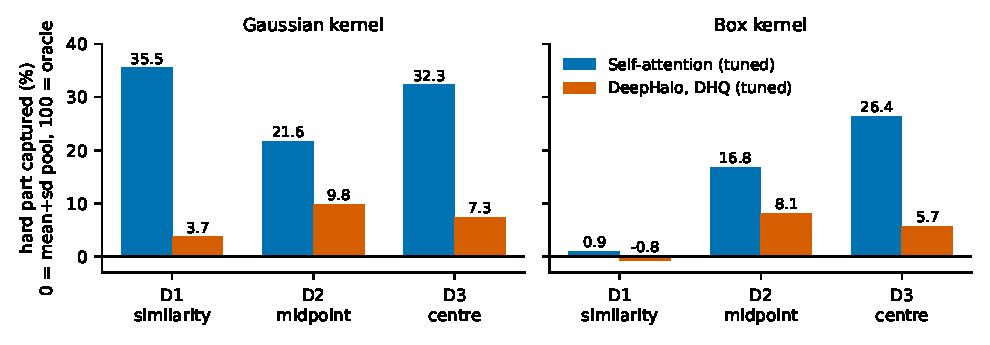
\includegraphics[width=\textwidth]{figs/hard_part.pdf}
\caption{Share of the hard part captured by the tuned models (synth\_final runs, 30 seeds, 0--29). Left: Gaussian kernel. Right: box kernel, where attention has no built-in shortcut.}\label{fig:hard}
\end{figure}

Two things stand out. First, attention captures much more of the hard part: 16.8\% to 32.3\% on the second- and third-order datasets, against 5.7\% to 9.8\% for DeepHalo. Second, even the better model is far from the oracle; most of the hard part is still not learned by anyone.

\subsection{Robustness: does the kernel matter?}\label{sec:8.6}

While analysing the results, we noticed that the Gaussian kernel can be written in a form that looks like the $\exp(\mathbf q\cdot\mathbf k)$ term inside softmax attention. This means attention may get a built-in shortcut for Gaussian similarity that has nothing to do with learning context in general. To test this, we repeated the experiments with the box kernel, which has no such form.

The result was clear. On similarity, attention's big lead on D1 (35.5\% against 3.7\%) \textbf{disappears} on D1b, where attention captures 0.9\% and DeepHalo $-$0.8\%. In other words, neither tuned model learns box-kernel similarity in any useful amount (the best model in our earlier sweep, 1-layer attention, captures only 3.8\%), so attention's success on D1 most likely came from the Gaussian kernel. On the second- and third-order datasets, however, attention's advantage \textbf{survives} the change of kernel (D2b: 16.8\% against 8.1\%; D3b: 26.4\% against 5.7\%). So the higher-order result is not a kernel trick.

\subsection{Depth or width?}\label{sec:8.7}

To see which part of the attention model matters, we compared a 2-layer attention model with a 1-layer model made wider (width 46) so that the two have a similar number of parameters. The 2-layer model won on D2 and on D3 on \textbf{all 30 seeds}. So the gain comes from \textbf{depth}, not from extra parameters. This fits well with the idea that each extra layer lets attention combine information from more items.

\subsection{Tuning barely changed the gap to the oracle}\label{sec:8.8}

After tuning over 22 configurations, the test losses of the best models moved only a little compared with the earlier, untuned models, and bigger or deeper models did not close the gap to the oracle. This pointed to a limit of data rather than of capacity, which the training-size sweep below confirms.

\subsection{Training-set size: the remaining gap is a data limit}\label{sec:8.9}

The gap to the oracle closes steadily as training data grows, with no sign of levelling off; below about 100,000 slates, no model learns higher-order context at all. The sweep trained the tuned self-attention model, the tuned DeepHalo model, the mean+sd pool and the twin on D0, D2, D3, D2b and D3b with 11,000, 30,000, 100,000, 285,000 and 1,000,000 training slates. Validation and test sets were identical at every size, smaller training sets were subsets of larger ones, and each size used 30 seeds (10 at 1,000,000). The 285,000 row reuses the final run of Section 8.5.

\begin{figure}[H]
\centering
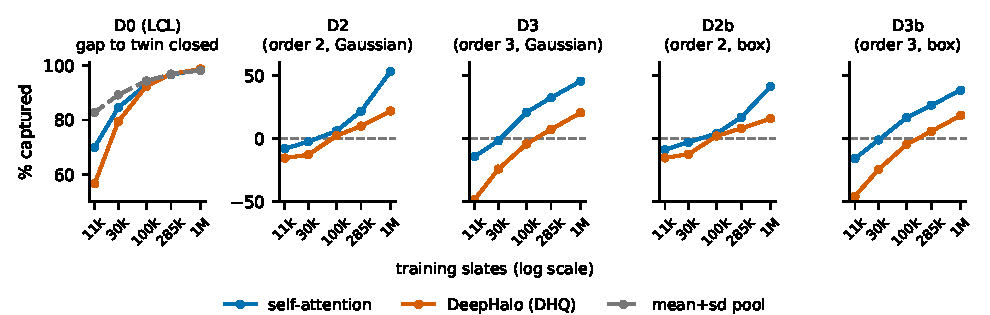
\includegraphics[width=\textwidth]{figs/size_sweep.pdf}
\caption{Share captured against training-set size (mean over 30 seeds, 10 at 1,000,000). D0: share of the whole context effect (gap to twin closed); other panels: share of the hard part, where 0 is the mean+sd pool.}\label{fig:size}
\end{figure}

Four observations follow from the sweep:

\begin{enumerate}
\item \textbf{More data keeps helping.} On D2, self-attention captures $-$8.1\% of the hard part at 11,000 slates, 21.6\% at 285,000 and 53.1\% at 1,000,000. Since larger and deeper models did not help (Section 8.8) while more data did, the remaining gap to the oracle is mainly a limit of data, not of architecture.
\item \textbf{Below about 100,000 slates, higher-order context is not learnable.} At 11,000 and 30,000 slates, both models do, on average, \emph{worse} than the mean+sd pool on every higher-order dataset (negative values): trying to model the higher-order effect costs more than it gains. Self-attention first beats the pool on every seed at 100,000 slates.
\item \textbf{Self-attention needs less data than DeepHalo, and its lead grows with data.} At 100,000 slates, DeepHalo is still below the pool on D3 and D3b while self-attention captures 20.8\% and 16.6\%. At 1,000,000 slates, self-attention captures 53.1\% against 21.8\% on D2 and 45.4\% against 20.4\% on D3; the same pattern holds with the box kernel.
\item \textbf{First-order linear context favours the simplest model when data are scarce.} On D0 the mean+sd pool, whose averaging matches the LCL form exactly, closes 82.8\% of the gap to the twin at 11,000 slates against 70.0\% for self-attention and 56.6\% for DeepHalo. All three converge to about 97\% at 285,000 and about 98.5\% at 1,000,000, where none is reliably better than another.
\end{enumerate}

\subsection{Lessons learned along the way}\label{sec:8.10}

We want to be honest that some of our early conclusions did not survive careful checks:

\begin{itemize}
\item Our first claim that attention beats DeepHalo everywhere was partly because we used the weaker linear version of DeepHalo.
\item The similarity advantage on D1 most likely came from the Gaussian kernel (Section 8.6).
\item An early claim that DeepHalo never goes beyond the mean+sd summary was false for the quadratic version.
\end{itemize}

Each of these was corrected by adding a control or a check, and all the numbers in this section are from the corrected, final runs.

\subsection{Real data: LPMC and Expedia}\label{sec:8.11}

On two real datasets, self-attention finds no usable context in London travel-mode choice (LPMC) and a small but reliable context gain in Expedia hotel bookings. Most of the Expedia gain is also captured by a simple within-slate normalisation of features. Neither dataset gives reliable evidence of context beyond such low-order slate statistics at the sample sizes available.

\textbf{Data.} The same model families and controls as in the synthetic study were applied to both datasets.

\begin{table}[H]
\centering\small
\caption{The two real datasets.}\label{tab:6}
\begin{tabularx}{\textwidth}{@{}>{\raggedright\arraybackslash}X>{\raggedright\arraybackslash}X>{\raggedright\arraybackslash}X@{}}
\toprule
 & \textbf{LPMC} & \textbf{Expedia} \\
\midrule
Choice & Travel mode of a trip: walk, cycle, public transport or drive & Hotel booked in a search \\
Alternatives per choice set & 4, all always available & 5 to 38 (mean 23.8) \\
Features & 8 per mode, plus 17 traveller features & 14 per hotel, plus 10 search features \\
Sample & 81,086 trips & 15,845 searches with exactly one booking, from randomised rankings only (\texttt{random\_bool}${}=1$) \\
Split (train / val / test) & Survey years 1--2 for training and validation (validation = 10\% of households), year 3 for testing: 49,327 / 5,439 / 26,320 & By time, latest searches for testing: 11,092 / 1,584 / 3,169 \\
\bottomrule
\end{tabularx}
\end{table}

Two preparation choices matter for interpretation. On LPMC, the split holds out whole households and a whole survey year, so no traveller appears in both training and test. On Expedia, every model includes a separate learned position term, so a context gain cannot come from the position of a hotel on the page. The historical-price feature was also dropped, because it becomes zero for every hotel in the final four weeks of the data.

\textbf{LPMC: no detectable context.} Test negative log-likelihood (NLL) on the held-out year, mean $\pm$ standard deviation over seeds:

\begin{table}[H]
\centering\small
\caption{LPMC: test NLL on the held-out survey year (mean $\pm$ s.d. over seeds).}\label{tab:7}
\begin{tabular}{@{}llll@{}}
\toprule
\textbf{Model} & \textbf{Parameters} & \textbf{Seeds} & \textbf{Test NLL} \\
\midrule
MNL (attributes and mode constants) & --- & 1 & 0.8843 \\
MNL with mode-specific traveller effects & --- & 1 & 0.7242 \\
DeepHalo, released code ($L=4$, $d=32$, $H=8$) & 42,369 & 5 & 0.6881 $\pm$ 0.0021 \\
Context-free MLP & 19,969 & 5 & 0.6835 $\pm$ 0.0036 \\
Context-free MLP, size-matched & 9,606 & 5 & 0.6822 $\pm$ 0.0004 \\
DeepHalo, size-matched ($d=15$) & 10,188 & 5 & 0.6805 $\pm$ 0.0025 \\
Self-attention, blindfolded twin & 9,473 & 15 & 0.6797 $\pm$ 0.0034 \\
Self-attention (1 layer, $d=32$, 2 heads) & 9,473 & 15 & 0.6790 $\pm$ 0.0030 \\
\bottomrule
\end{tabular}
\par\vspace{2pt}{\footnotesize Parameter counts for DeepHalo are the parameters actually used; the released code also defines two unused linear maps (2,112 and 480 extra parameters).}
\end{table}

Over 15 paired seeds, self-attention minus its twin is $-$0.0007 $\pm$ 0.0012 (standard error), and self-attention is better on only 9 of 15 seeds. Seeing the other modes therefore adds nothing measurable. This is plausible for LPMC: all four modes are always available, so the choice set never changes in composition, and context can act only through the attributes of the other modes.

We also checked our DeepHalo against the paper. On a random 80/10/10 row split, which we believe is the paper's protocol, DeepHalo reached a test NLL of 0.6404 $\pm$ 0.0016 over 5 seeds, against 0.6407 reported in the paper, so the reproduction is close. On the same split, however, our context-free MLP reached 0.6382 $\pm$ 0.0006, whereas the paper reports 0.6870 $\pm$ 0.0049 for its MLP baseline. The advantage of DeepHalo over a context-free model reported on LPMC is therefore not reproduced here. One possible reason is that our MLP receives the traveller features; the inputs of the paper's MLP baseline should be checked before drawing a firm conclusion.

\textbf{Expedia: a reliable but shallow context gain.} Test NLL on the latest searches (a uniform guess scores 3.0282):

\begin{table}[H]
\centering\small
\caption{Expedia: test NLL on the latest searches (mean $\pm$ s.d. over seeds).}\label{tab:8}
\begin{tabularx}{\textwidth}{@{}>{\raggedright\arraybackslash}Xlll@{}}
\toprule
\textbf{Model} & \textbf{Parameters} & \textbf{Seeds} & \textbf{Test NLL} \\
\midrule
Position only & --- & 1 & 2.8373 \\
MNL & 55 & 1 & 2.6343 \\
DeepHalo at the paper's Expedia size ($L=5$, $d=32$) & about 52,000 & 5 & 2.6069 $\pm$ 0.0102 \\
LCL & --- & 1 & 2.5965 \\
Context-free MLP, size-matched & 9,562 & 5 & 2.5791 $\pm$ 0.0060 \\
Self-attention, blindfolded twin & 9,482 & 15 & 2.5761 $\pm$ 0.0038 \\
Pool: own features + others' mean & 9,522 & 15 & 2.5719 $\pm$ 0.0042 \\
Pool: own features + others' mean and sd & 9,588 & 15 & 2.5693 $\pm$ 0.0046 \\
Pool: + own features standardised against others (z-score) & 9,358 & 15 & 2.5617 $\pm$ 0.0053 \\
DeepHalo, tuned (quadratic, $L=4$, $d=6$, $H=8$) & 2,162 & 15 & 2.5585 $\pm$ 0.0072 \\
Self-attention (1 layer, $d=32$, 2 heads) & 9,482 & 15 & 2.5584 $\pm$ 0.0056 \\
\bottomrule
\end{tabularx}
\end{table}

Four results stand out:

\begin{enumerate}
\item \textbf{Context is present.} Self-attention beats its blindfolded twin by 0.0177 $\pm$ 0.0017 nats and is better on all 15 seeds. DeepHalo also gains from context, by 0.0092 $\pm$ 0.0023 nats against its own blindfolded version.
\item \textbf{Tuned against tuned, the two architectures tie.} DeepHalo at the paper's size overfits badly (0.0278 nats worse than a context-free MLP), and its best configurations are very small. After tuning both families, self-attention (width 24, 5,586 parameters) minus tuned DeepHalo is $-$0.0032 $\pm$ 0.0023, which is within noise.
\item \textbf{Most of the context is simple normalisation.} A pooled model that sees each hotel's features standardised against the other hotels in the same search recovers 0.0144 of self-attention's 0.0177-nat gain over the twin, about 81\%. The remainder, $-$0.0034 $\pm$ 0.0020, is not significant at the two-standard-error level. A similarity-weighted pool adds nothing significant beyond the mean and sd ($-$0.0018 $\pm$ 0.0020).
\item \textbf{The model's responses are partly competitor-specific.} When the price of one competitor is cut by 10\%, self-attention lowers the scores of the hotels closest to it in price the most, and raises those of the most distant ones. Pooled controls show a similar pattern, so this alone does not prove pairwise comparison. However, when the cut is applied to one of two different competitors in the same search, self-attention's responses differ between the two cases almost three times as much as those of the pooled model (spread 0.0125 against 0.0046), while LCL's do not differ at all. This is suggestive, though not conclusive, evidence of item-to-item comparison.
\end{enumerate}

\textbf{What this says about higher orders.} On both datasets, nothing beyond low-order slate statistics is reliably detected. This should not be read as proof that real choices contain no higher-order context effects. The Expedia training set has 11,092 searches, close to the smallest size (11,000) in the synthetic training-size sweep of Section 8.9. In that sweep, at 11,000 slates both models do worse than the mean+sd pool on every planted higher-order effect (self-attention captures $-$8.1\% to $-$15.8\% of the hard part). A higher-order effect of the size planted in this study would therefore be invisible with this much data, so the Expedia result reflects the limits of the data, not the absence of the effect.

\subsection{A first look inside the models}\label{sec:8.12}

On first-order LCL data, every model recovers the true parameters almost exactly, and self-attention does this by simply averaging the slate. On higher-order data, the attention heads pick out the items that are close in the two context features, mainly in the second layer. A direct IIA test ranks the models in the same order as our loss-based metric.

For this analysis we retrained four models on D0, D2 and D3 with 5 seeds (0--4), this time saving their weights: the tuned 3-layer self-attention model, a 1-layer self-attention model (width 32, 2 heads), the tuned DeepHalo model and the mean+sd pool. The data, seeds and training recipe were the same as in the final run, and the retrained models reproduced the final test losses exactly (difference 0.000). All numbers below are on the 50,000 test slates, as mean $\pm$ standard error over the 5 seeds.

\textbf{Recovering $\boldsymbol\theta$ and $A$ on LCL data.} For each trained model, we fitted the LCL form $u_i=\boldsymbol\theta\cdot\mathbf x_i+\mathbf x_i^{\top}A\,\bar{\mathbf x}_S$ to the model's own utilities and compared the fitted $\boldsymbol\theta$ and $A$ with the true ones. (On the true utilities, this fit recovers $\boldsymbol\theta$ and $A$ exactly, which confirms the procedure.)

\begin{table}[H]
\centering\small
\caption{Recovering $\boldsymbol\theta$ and $A$ from the trained models on D0 (5 seeds).}\label{tab:9}
\begin{tabularx}{\textwidth}{@{}>{\raggedright\arraybackslash}X>{\raggedright\arraybackslash}X>{\raggedright\arraybackslash}X>{\raggedright\arraybackslash}X>{\raggedright\arraybackslash}X@{}}
\toprule
\textbf{Model} & \textbf{Share of utility explained by the LCL form ($R^2$)} & \textbf{Correlation of fitted $A$ with true $A$} & \textbf{Size of fitted $A$ (1 = true size)} & \textbf{Cosine of fitted $\boldsymbol\theta$ with true $\boldsymbol\theta$} \\
\midrule
Self-attention, 3 layers (tuned) & 0.994 $\pm$ 0.001 & 0.999 & 0.955 $\pm$ 0.008 & 1.000 \\
Self-attention, 1 layer & 0.995 & 0.999 & 0.954 $\pm$ 0.004 & 1.000 \\
DeepHalo, quadratic (tuned) & 0.995 & 0.999 & 0.991 $\pm$ 0.015 & 1.000 \\
Mean+sd pool & 0.996 & 0.999 & 0.962 $\pm$ 0.010 & 1.000 \\
\bottomrule
\end{tabularx}
\end{table}

So, with 285,000 training slates, all four models have learned the LCL mechanism itself and not only good predictions: the pattern of $A$ is reproduced almost perfectly. The attention models estimate the context effect about 4--5\% too small, which is a mild shrinkage. This is much better recovery than in our earlier LCL experiments, which used 20,000 slates, and it agrees with the training-size sweep of Section 8.9.

\textbf{Where the context is computed.} We changed the attention of one layer at a time, in two ways: replacing it with a plain average over all items (``uniform''), or letting each item attend only to itself (``self''). The table shows the rise in test loss under the uniform change, as a percentage of the model's context gain over its blindfolded twin.

\begin{table}[H]
\centering\small
\caption{Rise in test loss when attention is replaced by a plain average, as a share of the context gain over the blindfolded twin (5 seeds).}\label{tab:10}
\begin{tabularx}{\textwidth}{@{}>{\raggedright\arraybackslash}Xlll@{}}
\toprule
\textbf{Attention replaced by a plain average in} & \textbf{D0 (order 1, LCL)} & \textbf{D2 (order 2)} & \textbf{D3 (order 3)} \\
\midrule
3-layer model, layer 1 only & 1.9\% & 11.8\% & 21.6\% \\
3-layer model, layer 2 only & 0.4\% & 146.5\% & 21.5\% \\
3-layer model, layer 3 only & 0.9\% & 121.7\% & 41.2\% \\
3-layer model, all layers & 3.7\% & 252.7\% & 88.2\% \\
1-layer model & 3.1\% & 150.4\% & 82.1\% \\
\bottomrule
\end{tabularx}
\end{table}

On LCL data, averaging costs almost nothing, and the attention heads are in fact almost uniform: their spread is 0.98 to 0.99 on a scale where 1 means perfectly uniform, and each item puts about 0.10 (that is, 1/10) of its weight on itself. So for LCL, self-attention simply computes the mean of the slate, which is exactly what the LCL form needs. On D2 and D3, averaging costs a lot, so the model really needs selective attention there. In the 3-layer model, this selective attention sits mainly in layers 2 and 3 on D2, while layer 1 can be averaged at little cost. (The layer-3 value on D2 varies a lot across seeds, $\pm$ 94 percentage points.)

The ``self'' change gives a surprising result: it raises the loss by much more than the whole context gain, for example by 431\% of it for the 1-layer model on D0. The trained network depends on the information coming from other items, and when this information is removed its internal representation breaks, so it does worse than a twin that was trained without context from the start. The ``self'' change therefore measures how much the network depends on context, not how much context is worth, and the uniform change is the cleaner test of what attention contributes.

\textbf{What the heads attend to.} For each head, we computed the correlation between the attention weight from item $i$ to item $j$ and how close the two items are, once in the two context features and once in the other four features as a control. On D2, the heads of the 1-layer model have correlations of 0.58 and 0.51 with closeness in the context features, against $-$0.01 and $-$0.02 with closeness in the other features. In the 3-layer model the strongest correlations are in layer 2 (0.55 and 0.49), whose heads are also the least uniform (spread 0.72 and 0.83). On D3 the pattern is the same but weaker (1-layer: 0.47 and 0.35; 3-layer, layer 2: 0.38 and 0.26). So on higher-order data, the attention heads learn to look at the items that are close in exactly the features that define the planted effect. These datasets use the Gaussian kernel, which gives softmax attention a built-in shortcut (Section 8.6); Section 8.13 repeats the analysis on the box-kernel datasets and finds the same pattern.

\textbf{A direct IIA test.} For each test slate, we kept items 0 and 1, replaced the other 8 items with new random items, and measured how much $u_0-u_1$ changed, both under the true utilities and under the model. Under IIA this change would be zero. The table gives the correlation between the true and the model's changes, and the slope (1 means the model changes by the right amount).

\begin{table}[H]
\centering\small
\caption{Direct IIA test: correlation and slope between the true and the model's change in $u_0-u_1$ (5 seeds).}\label{tab:11}
\begin{tabularx}{\textwidth}{@{}>{\raggedright\arraybackslash}X>{\raggedright\arraybackslash}X>{\raggedright\arraybackslash}X>{\raggedright\arraybackslash}X@{}}
\toprule
\textbf{Model} & \textbf{D0: correlation / slope} & \textbf{D2: correlation / slope} & \textbf{D3: correlation / slope} \\
\midrule
Self-attention, 3 layers (tuned) & 0.980 / 0.949 & 0.689 / 0.556 & 0.887 / 0.830 \\
Self-attention, 1 layer & 0.983 / 0.948 & 0.636 / 0.455 & 0.860 / 0.762 \\
DeepHalo, quadratic (tuned) & 0.988 / 0.987 & 0.614 / 0.456 & 0.831 / 0.773 \\
Mean+sd pool & 0.984 / 0.958 & 0.553 / 0.340 & 0.827 / 0.710 \\
\bottomrule
\end{tabularx}
\end{table}

On LCL data all models pass this test almost perfectly. On D2 and D3 the 3-layer attention model is best, the 1-layer model and DeepHalo come next, and the pool is last, which is the same order as the hard-part results of Section 8.5. The deeper attention model also beats the 1-layer one, in line with the depth result of Section 8.7. All slopes are below 1, so every model under-reacts to a change of context, most of all on D2. The pool still scores fairly well on D3 (correlation 0.827), because, as explained in Section 9.1, a large part of a third-order effect can be imitated by the mean and standard deviation of the slate.

\subsection{The look inside, checked on the box kernel and with 10 seeds}\label{sec:8.13}

The findings of Section 8.12 hold on box-kernel data, where attention has no built-in shortcut, so the attention heads really do learn to look at nearby items. Before running this check, we wrote down that if the box-kernel models did not show this pattern, the Gaussian result would have to be explained by the shortcut of Section 8.6. That did not happen.

We repeated every analysis of Section 8.12 on five datasets (D0, D2, D3 and the box-kernel D2b, D3b) with 10 seeds each. The retrained models again reproduced the final-run test losses exactly. The main numbers are:

\begin{itemize}
\item \textbf{Recovering $\boldsymbol\theta$ and $A$ on LCL data (10 seeds):} the fitted $A$ still matches the true $A$ with correlation 0.999 for every model. Its size is 0.986 $\pm$ 0.008 of the true size for DeepHalo, 0.964 $\pm$ 0.006 for 3-layer attention, 0.961 $\pm$ 0.004 for 1-layer attention and 0.966 $\pm$ 0.006 for the pool. These are very close to the 5-seed values.
\item \textbf{Attention follows closeness, also on box data:} for the 1-layer model, the correlation between attention weight and closeness in the two context features is 0.59 and 0.60 (two heads) on D2b, against 0.61 and 0.53 on Gaussian D2, and 0.42 and 0.39 on D3b, against 0.44 and 0.37 on D3. Closeness in the other four features stays near zero everywhere (between $-$0.03 and 0.00). In the 3-layer model, the strongest focusing is again in layer 2 (0.48 and 0.46 on D2b).
\item \textbf{Where the context is computed, on box data:} replacing attention by a plain average costs, as a share of the context gain, 14\% in layer 1, 146\% in layer 2 and 142\% in layer 3 on D2b, and 15\%, 24\% and 47\% on D3b. This is the same pattern as on the Gaussian datasets.
\item \textbf{IIA test on box data:} the order of the models is unchanged. On D2b the correlation / slope is 0.624 / 0.477 for 3-layer attention, 0.573 / 0.368 for 1-layer attention, 0.563 / 0.395 for DeepHalo and 0.504 / 0.297 for the pool; on D3b it is 0.864 / 0.789, 0.835 / 0.735, 0.806 / 0.752 and 0.801 / 0.679.
\end{itemize}

\subsection{Depth and the order of interaction: a first test}\label{sec:8.14}

In practice, two layers of full self-attention are enough for effects of order 2 to 5, and attention without its feed-forward network learns very little context; a clean test of how depth limits the order was therefore inconclusive.

\textbf{Design.} We created two more datasets, D4 and D5, in which an item gains utility when it is close to the centre of \emph{four} or \emph{five} other items. Their strength was calibrated with the usual rule (hard part 0.03 nats):

\begin{table}[H]
\centering\small
\caption{Calibration of the order-4 and order-5 datasets.}\label{tab:12}
\begin{tabularx}{\textwidth}{@{}lll>{\raggedright\arraybackslash}X>{\raggedright\arraybackslash}X@{}}
\toprule
\textbf{Dataset} & \textbf{Order} & \textbf{$\lambda$} & \textbf{Total context effect (twin gap)} & \textbf{Share explained by the slate's mean and sd} \\
\midrule
D4 & 4 & 0.144 & 0.108 nats & 72.2\% \\
D5 & 5 & 0.110 & 0.112 nats & 73.2\% \\
\bottomrule
\end{tabularx}
\end{table}

The last column continues the concentration effect: about 30\% of the effect is explained by simple slate statistics at order 2, about 61\% at order 3 and about 72--73\% at orders 4 and 5 (these are the calibration values; in the final runs the trained pool closes 31\% of the twin gap on D2 and 70\% on D3). On D2 to D5 we trained three families at depths 1 to 4, with the number of parameters fixed within each family, 5 seeds and 285,000 training slates. The \emph{full self-attention} family is our model of Section 5 (about 26,000 parameters; width 56, 40, 32 and 28 at depths 1 to 4). The two \emph{attention-only} families have a per-item MLP embedding followed only by attention layers with residual connections, with softmax or with linear attention (about 16,000 parameters; width 56, 42, 34 and 30). The idea behind this test is a simple counting argument of our own, not yet checked against the literature. In a network made only of linear attention layers, each layer can combine what an item already knows with what other items already know, so the number of other items that can act together on one item's utility grows from 1 after one layer to 3 after two layers and to at most $2^L-1$ after $L$ layers. A nonlinear feed-forward layer between attention steps can raise the order by itself (for example, squaring a sum over items gives terms that depend on pairs of items), so this counting holds only for attention-only models.

\textbf{What we expected.} Before the runs, we wrote that linear attention-only models should reach order at most $2^L-1$ (1, 3, 7, 15), so that the 1-layer model would capture little and the 2-layer model should work on orders 2 and 3 but less on 4 and 5; that softmax attention-only models should improve with depth; and that full self-attention should improve with depth up to about 3 layers.

\textbf{Results.} Percentage of the hard part captured (0 = mean+sd pool, 100 = oracle), mean over 5 seeds:

\begin{table}[H]
\centering\small
\caption{Percentage of the hard part captured against depth (mean over 5 seeds).}\label{tab:13}
\begin{tabular}{@{}llllll@{}}
\toprule
\textbf{Family} & \textbf{Dataset (order)} & \textbf{$L=1$} & \textbf{$L=2$} & \textbf{$L=3$} & \textbf{$L=4$} \\
\midrule
Full self-attention & D2 (2) & 13.6 & 21.3 & 23.9 & 23.5 \\
Full self-attention & D3 (3) & 18.1 & 30.5 & 30.0 & 32.2 \\
Full self-attention & D4 (4) & 21.6 & 40.7 & 42.1 & 42.3 \\
Full self-attention & D5 (5) & 22.8 & 40.6 & 41.8 & 42.1 \\
Attention-only, softmax & D2 (2) & $-$15.4 & $-$0.9 & 3.2 & 3.7 \\
Attention-only, softmax & D3 (3) & $-$78.6 & $-$25.4 & $-$5.0 & 4.2 \\
Attention-only, softmax & D4 (4) & $-$213.6 & $-$46.5 & $-$33.8 & $-$10.5 \\
Attention-only, softmax & D5 (5) & $-$348.8 & $-$78.9 & $-$57.5 & $-$42.1 \\
Attention-only, linear & D2 (2) & $-$5.2 & $-$0.4 & 0.7 & $-$2.0 \\
Attention-only, linear & D3 (3) & $-$69.1 & $-$22.9 & $-$19.4 & $-$16.8 \\
Attention-only, linear & D4 (4) & $-$219.2 & $-$77.1 & $-$61.2 & $-$79.0 \\
Attention-only, linear & D5 (5) & $-$407.0 & $-$185.0 & $-$146.9 & $-$140.4 \\
\bottomrule
\end{tabular}
\end{table}

Standard errors are mostly between 1 and 3 points for full self-attention and larger for the attention-only models (up to 27 points). No run failed numerically.

\begin{figure}[H]
\centering
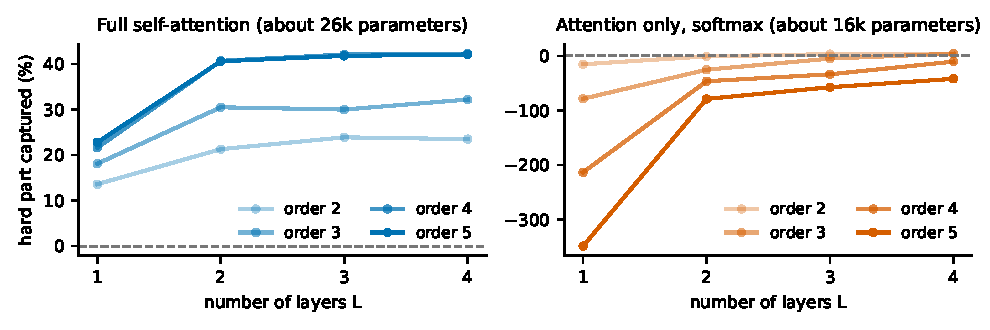
\includegraphics[width=0.85\textwidth]{figs/depth.pdf}
\caption{The results of Table~\ref{tab:13} as a picture: hard part captured against depth for effects of order 2 to 5 (mean over 5 seeds). Darker lines are higher orders.}\label{fig:depth}
\end{figure}

Three points come out of this:

\begin{enumerate}
\item \textbf{For full self-attention, the second layer matters and further layers do not.} At every order, going from 1 to 2 layers gives a large gain, and 3 or 4 layers add little. Even a 1-layer model captures part of an order-5 effect, which fits the point above that the feed-forward network after attention can itself raise the order. The gain from the second layer grows with the order (7.7 points at order 2, 12.4 at order 3, 19.1 at order 4 and 17.8 at order 5), so higher orders do benefit more from depth, but we see no doubling pattern of the kind $2^L-1$.
\item \textbf{Attention without its feed-forward network learns very little context.} Both attention-only families are worse than the simple mean+sd pool almost everywhere, and the deficit grows with the order, because the low-order part of the effect also grows with the order and these models fail to capture even that part. Softmax attention improves with depth and only just becomes positive at depth 3 to 4 on order 2 and at depth 4 on order 3. Linear attention never clearly beats the pool, not even with 2 layers on order 2, where by our counting it has enough capacity.
\item \textbf{The test of $2^L-1$ is therefore inconclusive.} Because the attention-only models do not learn even the easy part of the effect, we cannot see whether their limit follows the predicted orders. We cannot yet tell whether this failure is about what these models can represent or about how hard they are to train: they have no LayerNorm and fewer parameters (about 16,000 against 26,000). The link between depth and order for attention therefore remains a hypothesis; a fair test would need attention-only models that at least match the pool, for example with normalisation, more parameters or more data.
\end{enumerate}

\section{Discussion and an early theory}

\subsection{What the results tell us so far}\label{sec:9.1}

Putting the results together, we can answer our two questions in a careful way:

\begin{itemize}
\item \textbf{Does self-attention capture context effects?} Yes for first-order linear context, almost fully (about 97\%). For higher-order context, only partly: it captures between about a sixth and a third of the hard part, and no model learns box-kernel similarity in any useful amount.
\item \textbf{Does it do better than DeepHalo?} On first-order linear context, no; they tie. On second- and third-order context, yes, on every seed and with both kernels. This is interesting because DeepHalo was designed for higher-order effects.
\end{itemize}

A useful observation is the \textbf{concentration effect}. The midpoint of two random items, or the centre of three, tends to lie close to the centre of the whole slate. The more items we average, the closer these points crowd together. So part of a higher-order effect can be imitated by simple low-order statistics of the slate, like the mean. This is why we measure the \emph{hard part} beyond mean+sd, and it also explains why some models look good on raw loss without really learning the higher-order structure.

\subsection{Limitations}\label{sec:9.2}

\begin{itemize}
\item All the results above are on \textbf{synthetic data} with 10 items and 6 features. Real slates are larger and noisier.
\item In the main comparison we have tested orders 1, 2 and 3 only (orders 4 and 5 appear only in the depth test of Section 8.14), each on its own. Real data will contain a \textbf{mix of orders} together.
\item Our main metric is based on average loss. The direct IIA test and the look inside the models (Sections 8.12 and 8.13) support it, but they were run on 5 and 10 seeds rather than the 30 of the main results.
\item Higher-order context needs large data: below about 100,000 slates no model learned it, so conclusions from smaller real datasets are limited to low-order context.
\end{itemize}

\section{Future work}

The next steps, in the order we plan to do them:

\begin{enumerate}
\item \textbf{Extend the training-size sweep} beyond 1,000,000 slates (Section 8.9) to find where the gain levels off, and repeat it on mixed-order data.
\item \textbf{Extend the IIA test and the attention analysis.} Run the analyses of Sections 8.12 and 8.13 on all 30 seeds, and add DeepHalo's own order-wise readout (relative context effects computed from subsets of the slate) to compare the two models order by order.
\item \textbf{Mixed-order data.} Build datasets that mix several orders at once, like real data, with partial oracles that know only some of the orders. This lets us see which orders a model picks up first.
\item \textbf{Real data.} Extend Section 8.11: compute DeepHalo-style order-wise relative context effects on the trained Expedia models, and use the training-size sweep to state how large a higher-order effect must be to be detectable with about 11,000 searches.
\item \textbf{Deeper interpretability.} Section 8.12 shows \emph{which} layers and heads carry the context. The next step is to explain \emph{how}: for example, whether the value and output weights of the attention, together with the readout layer, reproduce the matrix $A$ on LCL data. In earlier work we saw that reading the attention weights directly gives a very different picture from behavioural probing, and this analysis would help explain that difference.
\end{enumerate}

%======================================================== BIB
\addcontentsline{toc}{section}{References}
\section*{References}
\begin{multicols}{2}
\footnotesize
\renewcommand{\section}[2]{}
\setlength{\bibsep}{2pt}
\begin{thebibliography}{99}
\bibitem[Batsell and Polking(1985)]{batsell1985} Batsell, R. R. and Polking, J. C. (1985). A new class of market share models. \emph{Marketing Science}, 4(3):177--198.
\bibitem[Bradley and Terry(1952)]{bradley1952} Bradley, R. A. and Terry, M. E. (1952). Rank analysis of incomplete block designs: I. The method of paired comparisons. \emph{Biometrika}, 39(3/4):324--345.
\bibitem[Evers and Lakens(2014)]{evers2014} Evers, E. R. K. and Lakens, D. (2014). Revisiting Tversky's diagnosticity principle. \emph{Frontiers in Psychology}, 5:875.
\bibitem[Goldstone et~al.(1997)]{goldstone1997} Goldstone, R. L., Medin, D. L., and Halberstadt, J. (1997). Similarity in context. \emph{Memory \& Cognition}, 25(2):237--255.
\bibitem[Huber et~al.(1982)]{huber1982} Huber, J., Payne, J. W., and Puto, C. (1982). Adding asymmetrically dominated alternatives: Violations of regularity and the similarity hypothesis. \emph{Journal of Consumer Research}, 9(1):90--98.
\bibitem[Kajitsuka and Sato(2024)]{kajitsuka2024} Kajitsuka, T. and Sato, I. (2024). Are transformers with one layer self-attention using low-rank weight matrices universal approximators? In \emph{ICLR 2024}.
\bibitem[Luce(1959)]{luce1959} Luce, R. D. (1959). \emph{Individual Choice Behavior: A Theoretical Analysis}. Wiley.
\bibitem[McFadden(1974)]{mcfadden1974} McFadden, D. (1974). Conditional logit analysis of qualitative choice behavior. In \emph{Frontiers in Econometrics}, pages 105--142. Academic Press.
\bibitem[Pfannschmidt et~al.(2022)]{pfannschmidt2022} Pfannschmidt, K., Gupta, P., Haddenhorst, B., and H\"ullermeier, E. (2022). Learning context-dependent choice functions. \emph{International Journal of Approximate Reasoning}.
\bibitem[Pobrotyn et~al.(2020)]{pobrotyn2020} Pobrotyn, P., Bartczak, T., Synowiec, M., Bia{\l}obrzeski, R., and Bojar, J. (2020). Context-aware learning to rank with self-attention. In \emph{SIGIR eCom Workshop}.
\bibitem[Seshadri et~al.(2019)]{seshadri2019} Seshadri, A., Peysakhovich, A., and Ugander, J. (2019). Discovering context effects from raw choice data. In \emph{ICML 2019}, PMLR 97.
\bibitem[Simonson(1989)]{simonson1989} Simonson, I. (1989). Choice based on reasons: The case of attraction and compromise effects. \emph{Journal of Consumer Research}, 16(2):158--174.
\bibitem[Tomlinson and Benson(2021)]{tomlinson2021} Tomlinson, K. and Benson, A. R. (2021). Learning interpretable feature context effects in discrete choice. In \emph{KDD 2021}. arXiv:2009.03417.
\bibitem[Tversky(1972)]{tversky1972} Tversky, A. (1972). Elimination by aspects: A theory of choice. \emph{Psychological Review}, 79(4):281--299.
\bibitem[Tversky(1977)]{tversky1977} Tversky, A. (1977). Features of similarity. \emph{Psychological Review}, 84(4):327--352.
\bibitem[Tversky and Simonson(1993)]{tversky1993} Tversky, A. and Simonson, I. (1993). Context-dependent preferences. \emph{Management Science}, 39(10):1179--1194.
\bibitem[Vaswani et~al.(2017)]{vaswani2017} Vaswani, A., Shazeer, N., Parmar, N., Uszkoreit, J., Jones, L., Gomez, A. N., Kaiser, {\L}., and Polosukhin, I. (2017). Attention is all you need. In \emph{NeurIPS 30}.
\bibitem[Zhang et~al.(2025)]{zhang2025} Zhang, S., Wang, Z., Gao, R., and Li, S. (2025). DeepHalo: A neural choice model with controllable context effects. In \emph{NeurIPS 2025}. arXiv:2601.04616. Code: \url{github.com/Asimov-Chuang/DeepHalo}.
\end{thebibliography}
\end{multicols}

\end{document}
